% https://stackoverflow.com/a/59809988
\documentclass{beamer}

\usepackage{pgfplots}

\begin{document}

\begin{frame}
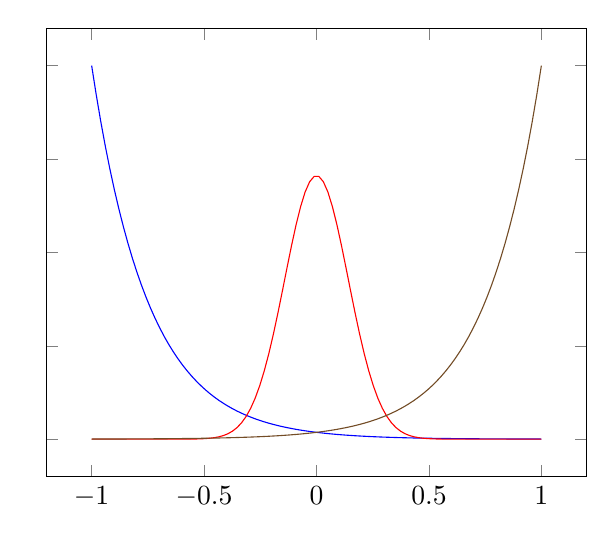
\begin{tikzpicture}
\begin{axis}[domain=-1:1,samples=100,yticklabels=\empty]
\addplot+[no markers] {4*exp(-4*(x+1))};
\addplot+[no markers] {1/sqrt(2*pi*0.02)*exp(-(x^2)/(2*0.02))};
\addplot+[no markers] {4*exp(4*(x-1))};
\end{axis}
\end{tikzpicture} 
\end{frame}

\end{document}
